\documentclass[11pt,a4paper]{article}
\pdfoutput=1

%=========================Package begin========================%
\usepackage{amsmath}
%\usepackage[english]{bable}
\usepackage{color}
\usepackage{multirow}
\usepackage{url}
\usepackage{cite}               % citiation
\usepackage{float}
\usepackage{graphicx, subfig}
\usepackage{geometry}
\usepackage{caption}
\usepackage{indentfirst}
\usepackage{times}              % set Times New Romans type
\usepackage{setspace}           % set line to line space 
%=========================Package end========================%
\geometry{left=2.5cm,right=2.5cm,top=2.5cm, bottom=2.5cm}

%=================================================================%
\newcommand{\HRule}[1]{\rule{\linewidth}{#1}}

\makeatletter
\def\printtitle{{\centering \@title\par}}
\makeatother

\makeatletter
\def\printauthor{{\centering \large \@author}}
\makeatother

\title{ \LARGE \textbf{{LOCld55 Design Document}}
        \HRule{2.5pt} \\[0.5cm]
        \normalsize \today
}

\author{
        \textbf{Author:} Wei Zhang\\
        \textbf{Co-author:} Di Guo, Quan Sun\\
        \textbf{}\\
        \textbf{Version} 1.1/July 4, 2018\\
        \textbf{}\\
        \textbf{Email:} \texttt{wzhang@mails.ccnu.edu.cn}\\
}
%=================================================================%

\begin{document}

%=================================================================%
\printtitle
\vfill                          % space from today to author

\printauthor
%=================================================================%
\begin{spacing}{1.25}           % set line to line space is 1.25


\thispagestyle{empty}           % first page doesn't page number

\newpage

\tableofcontents                % Create contents

\thispagestyle{empty}           % second page doesn't page number

\newpage

\setcounter{page}{1}

\section{LOCld55 Design Schedule}    % Part One
%=================================================================%
% add tabel
\begin{table}[H]
\centering
\caption{LOCld55 Design Schedule}

\begin{tabular}{|c|c|c|c|c|}
\hline
\multicolumn{1}{|c|}{\textbf{Item}} & \multicolumn{1}{c|}{\textbf{Subtask and description}} & \multicolumn{1}{c|}{\textbf{People}} & \multicolumn{1}{c|}{\textbf{Deadline}} & \multicolumn{1}{c|}{\textbf{Status}}\\
\hline
\multirow{2}{*}{Equalizer} & Design and Pre-simulation & Wei Zhang, Di Guo & Jun 5, 2018 & 100\% \\ \cline{2-5}
& Layout and Post-simulation & Wei Zhang, Di Guo & Jun 15, 2018 & 100\% \\
\hline
\multirow{2}{*}{LA} & Design and Pre-simulation & Wei Zhang, Di Guo & Jun 7, 2018 & 100\% \\ \cline{2-5}
& Layout and Post-simulation & Wei Zhang, Di Guo & Jun 16, 2018 & 100\% \\
\hline
\multirow{2}{*}{Output Driver} & Design and Pre-simulation & Wei Zhang, Di Guo & Jun 10, 2018 & 100\% \\ \cline{2-5}
& Layout and Post-simulation & Wei Zhang, Di Guo & Jun 20, 2018 & 100\% \\
\hline
\multirow{2}{*}{CCM biasing circuit} & Design and Pre-simulation & Wei Zhang, Di Guo & Jun 9, 2018 & 100\% \\ \cline{2-5}
& Layout and Post-simulation & Wei Zhang, Di Guo & Jun 20, 2018 & 100\% \\
\hline
\multirow{2}{*}{MOD biasing circuit} & Design and Pre-simulation & Wei Zhang, Di Guo & May 20, 2018 & 100\% \\ \cline{2-5}
& Layout and Post-simulation & Wei Zhang, Di Guo & Jun 30, 2018 & 0\% \\
\hline
\multirow{2}{*}{TOSA biasing circuit} & Design and Pre-simulation & Wei Zhang, Di Guo & May 25, 2018 & 100\% \\ \cline{2-5}
& Layout and Post-simulation & Wei Zhang, Di Guo & July 4, 2018 & 0\% \\
\hline
\multirow{3}{*}{Auto power control} & Investigate and Survey & Wei Zhang, Di Guo & July 6, 2018 & 0\% \\ \cline{2-5}
& Design and Pre-simulation & Wei Zhang, Di Guo & July 13, 2018 & 0\% \\ \cline{2-5}
& Layout and Post-simulation & Wei Zhang, Di Guo & July 20, 2018 & 0\% \\
\hline
\multirow{2}{*}{Receiver LA} & Design and Pre-simulation & Wei Zhang, Di Guo & July 25, 2018 & 0\% \\ \cline{2-5}
& Layout and Post-simulation & Wei Zhang, Di Guo & July 30, 2018 & 0\% \\
\hline
\multirow{2}{*}{Receiver Output buffer} & Design and Pre-simulation & Wei Zhang, Di Guo & Agust 3, 2018 & 0\% \\ \cline{2-5}
& Layout and Post-simulation & Wei Zhang, Di Guo & Agust 3, 2018 & 0\% \\
\hline
\multirow{2}{*}{I2C} & Design and Pre-simulation & Le Xiao & Agust 12, 2018 & 0\% \\ \cline{2-5}
& Layout and Post-simulation & Wei Zhang, Di Guo & Agust 16, 2018 & 0\% \\
\hline
\multirow{4}{*}{Final Integration} & Fill dummy & Wei Zhang, Di Guo & Agust 20, 2018 & 0\% \\ \cline{2-5}
& DRC Check & Wei Zhang, Di Guo & Agust 24, 2018 & 0\% \\ \cline{2-5}
& Pass LVS & Wei Zhang, Di Guo & Agust 28, 2018 & 0\% \\ \cline{2-5}
& Whole chip post-simulation & Wei Zhang, Di Guo & Sept 5, 2018 & 0\% \\ 
\hline
Generate gds file & gds file & Wei Zhang, Di Guo & Sept 10, 2018 & 0\% \\
\hline
\multirow{2}{*}{Document} & Write Design Document & Wei Zhang, Di Guo & Sept 30, 2018 & 0\% \\ \cline{2-5}
& Write User's manual & Wei Zhang, Di Guo & OCt 15, 2018 & 0\% \\
\hline

\end{tabular}
\end{table}

%=================================================================%
\newpage                            % newpage

\section{General Description of LOCld55}    % Part One

LOCld55 is a \textbf{single-channel, 14Gbps VCSEL driver} ASIC fabricated in SMIC 55nm CMOS technology specifically for datacom and telecommunication applications. The design follows the references\cite{ref1}. The output of the Laser Driver is intended to drive AC-coupled, edge-emitting, common-anode VCSEL. Modulation current and Bias current of Laser driver are adjusted via I2C Control Unit with reset function. The Limiting Amplifier Receiver with programmable bandwidth function is used to receive and amplify TIA's output signal then driver standard high serial interface. 

Figure 1 illustrates the block diagram of LOCld55 that includes a Laser Driver, I2C Control Unit, and Limiting Amplifier Receiver. The Laser Driver offers differential input and differential output interface with 800mV common-mode voltage.

%Figure 1: LOCld55 block diagram
\begin{figure}[H]
    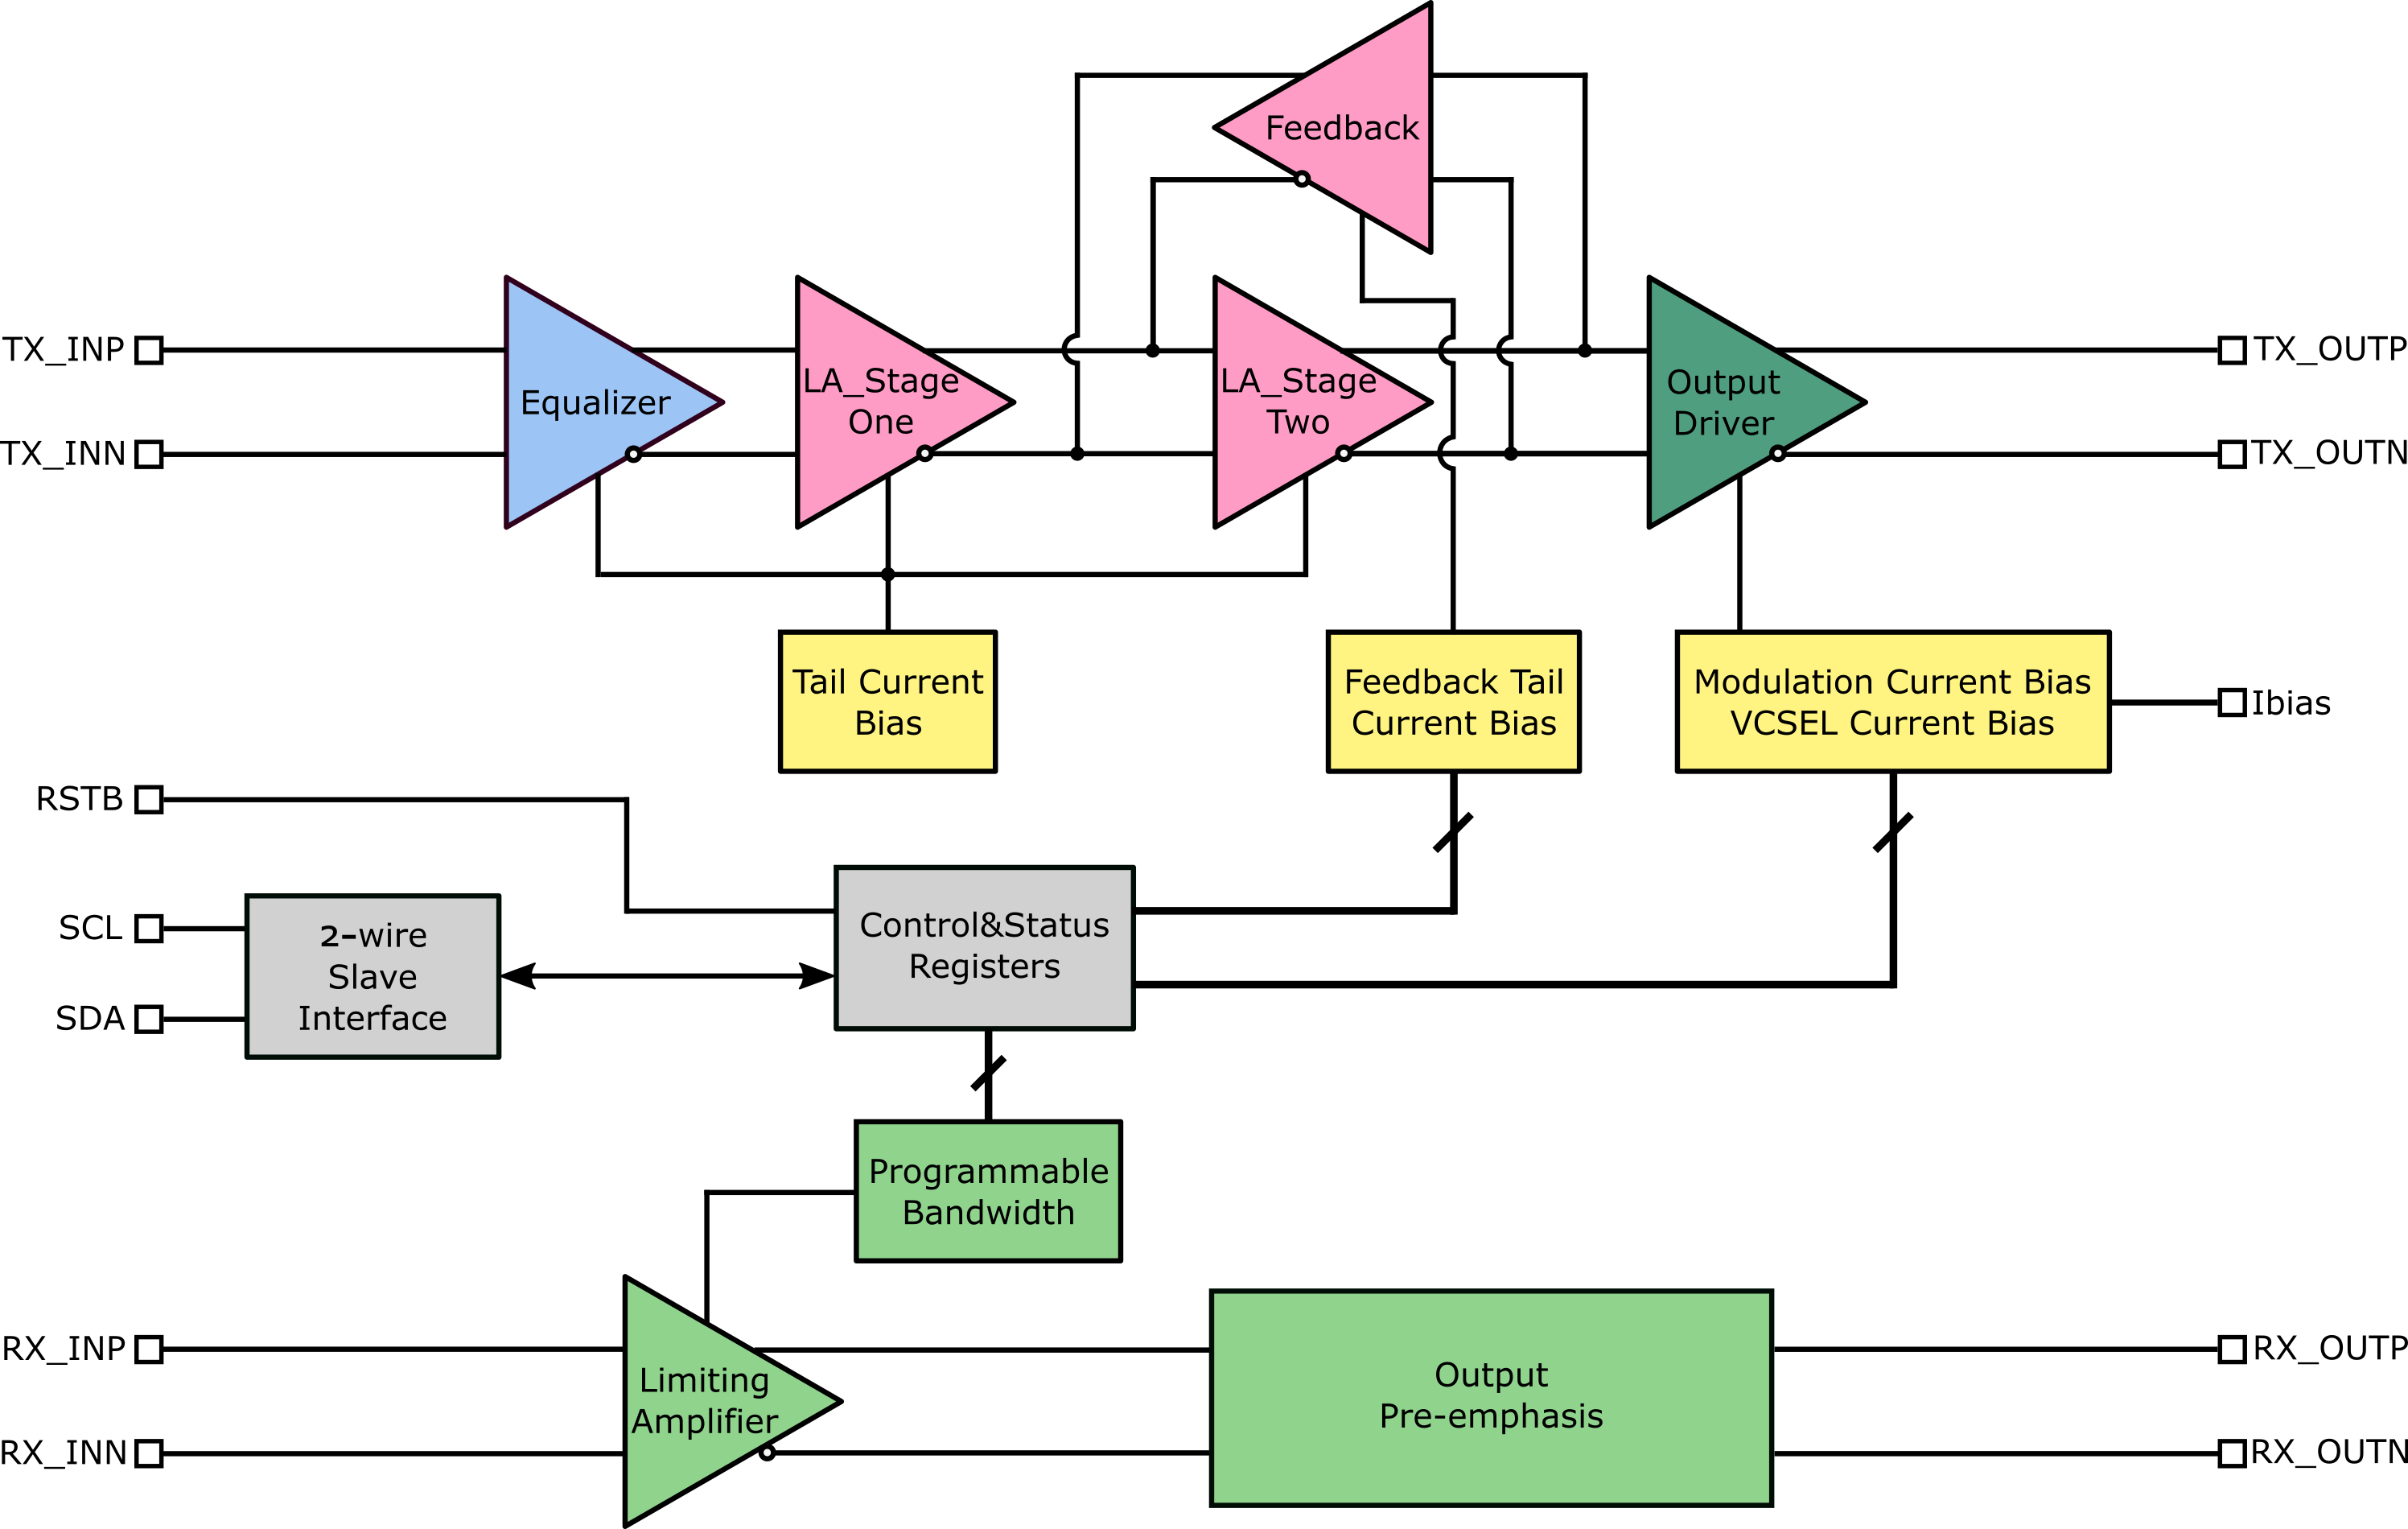
\includegraphics[width=\linewidth]{./Img/locld55.png}
    \caption{LOCld55 block diagram}
%    \lable{Figure 1}
\end{figure}
%Figure 1: LOCld55 block diagram

The die size and pad out of LOCld55 are shown in Section 2. Detailed schematic and layout designs are discussed in Section 3. The post-layout simulation results are introduced in Section 4.

\section{Pin Out of LOCld55}                % Part Two 
The top-level pin map and layout of LOCld are shown in Figure2.

\subsection{Pin Assignment}

\subsection{Pin Descriptions}

\section{Detailed design of LOCld55}        % Part Three
The overall schematic of LOCld55 is composed by single-channel module, receive side module and I2C module. The single-channel is composed of the Equalizer, the two-stage limiting amplifier, the output dirver, and their biasing circuits as shown in Figure 2. The single-channel layout (input traces and input/output pads are not included) is shown in Figure 3.

The biasing circuit is used to generate a feedback-control bias voltage for the tail current of the equalizer and two-stage limiting amplifier, so that the common voltage (0.8V) of each stage in equalizer and two-stage limiting amplifier is consistent under different corners and temperatures.

Output-driver biasing circuit receives control bits from I2C module and provides adjustable tail current for the output driver to change the modulation current and bias current for the TOSA.

Each module above will be detailly illustrated in the following sections.
%Figure 3: Layout single-channel
\begin{figure}[H]
    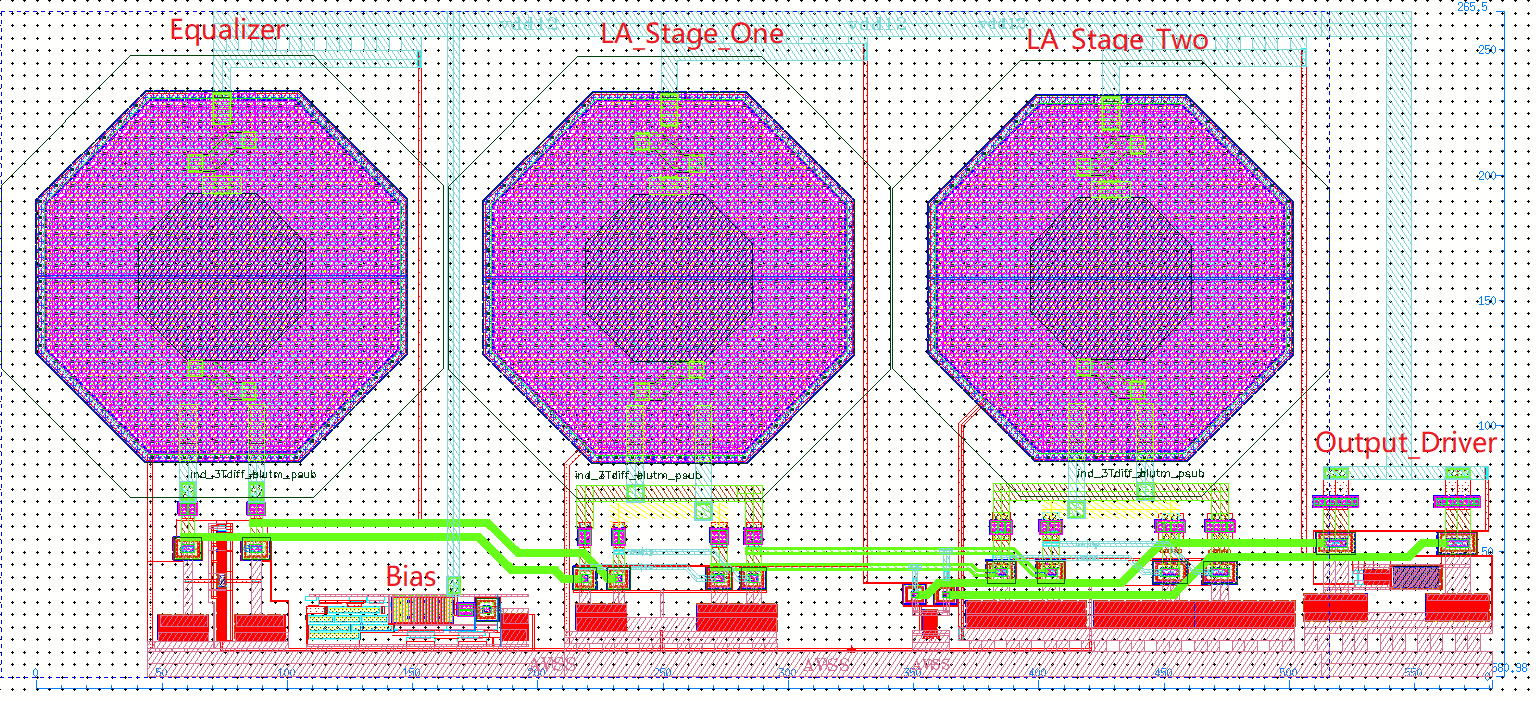
\includegraphics[width=\linewidth]{./Img/Layout_Eq_LA_OD_Background.png}
    \caption{Single-channel layout}
%    \lable{Figure 3}
\end{figure}
%Figure 3: Layout single-channel

\subsection{Equalizer}

The equalizer follows the previous input interface (0.8V common-voltage, single-ended 100mV amplitued).  

\subsection{Limited Amplifier (LA)}

\subsection{Output Driver (OD)}

\subsection{Equalizer and Limited Amplifier biasing circuit}

\subsection{Modulation biasing circuit and Current biasing circuit}

\subsection{I2C}

\section{LOCld55 simulation results}        % Part Four

\subsection{Equalizer simulation results}

\subsection{Limiting Amplifier simulation results}

%\section{References}                        % Part Five

\end{spacing}

\bibliographystyle{plain}
\addcontentsline{toe}{chapter}{References}
\bibliography{LOCld55_Design_Document}

\end{document}
